\chapter{基于GraphCodeBERT模型的智能合约漏洞检测}
\section{本章内容}
\label{sec:本章内容4}
本章是本文的核心内容,在上一章引入了智能合约的专家特征和语义特征后,本章将设计算法提取上述两种特征,然后参照GraphCodeBERT模型设计一个漏洞检测模型,最后开展实验。首先分别介绍了两种特征的计算或提取算法,然后介绍了GraphCodeBERT模型的基本架构、基于图的注意力掩码和两个关键的预训练任务,接着重点描述了一下本文提出的融合两种特征的方法。最后一部分介绍了实验的机器配置和模型的参数,以及用于对结果进行分析的评估指标,然后深入分析了实验结果。为了探究本文提出的专家特征以及特征融合等技术对实验结果的影响,最后还设计了多个消融实验并对结果进行了分析。
本章主要介绍了基于GraphCodeBERT模型的智能合约漏洞检测方法,并实验设计与结果。
\section{方法概述}
\label{sec:方法概述}
预训练模型可以学习并理解复杂的程序结构,并且具有跨语言通用性,大量工作表明预训练模型在漏洞检测任务中表现出色\cite{pretrained_is_good_1,pretrained_is_good_2,pretrained_is_good_3}。同时,Wu等人的研究表明预训练模型在识别智能合约的重入漏洞方面,明显优于当时最先进的方法\cite{wu2021peculiar}。遵循上述思路,本文拟采用GraphCodeBert模型为基础进行智能合约的漏洞检测研究。总的来说,本文的研究方法主要包含以下几个步骤:\textcircled{1}计算专家特征。依据xxx节描述的专家特征,从静态代码分析的角度对智能合约进行表示。\textcircled{2}构建语义图。依据xxx节描述的三种语义图,提取智能合约的语义信息。\textcircled{3}基于GraphCodeBERT训练漏洞检测模型。以GraphCodeBERT模型为基础,融合前两步生成的专家特征和语义信息训练漏洞检测模型。
\autoref{fig:framework}图xxx显示了本方法的框架结构。接下来,本文将逐一介绍上述三个步骤。
\begin{figure}[htbp]
    \centering
    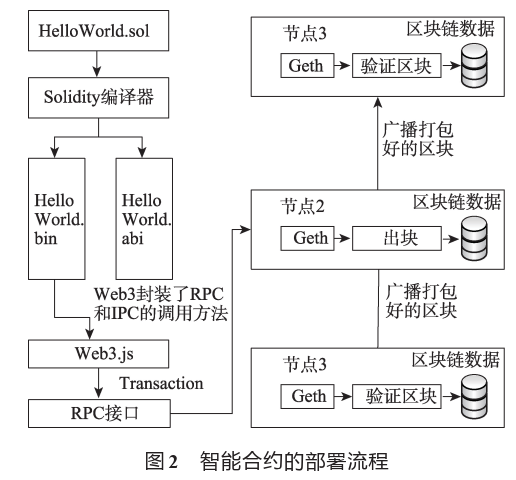
\includegraphics[width=.3\linewidth]{pictures/framework}
    \caption{\label{fig:framework}本方法的框架结构}
\end{figure}

\section{计算专家特征}
\label{sec:计算专家特征}
xxx节中获取的数据集并不包含合约的编译信息,为了获得xxx节中定义的专家特征,我们需要在本地编译Solidity源文件,然后构建抽象语法树再从中提取相关信息。py-solc-x\footnote{py-solc-x的网址}是solc\footnote{solc的网址}(Solidity编译器)的Python版本,py-solc-ast\footnote{py-solc-ast的网址}可以从solc编译后的信息中构建AST,并提供了API获取相关信息。

借助上述工具,我们提取出了xxx节中定义的基于静态代码度量的专家特征,其统计信息如\autoref{tab:new_dataset_statistics}所示。
\begin{table}[htbp]
    \caption{\label{tab:new_dataset_statistics}现有工作中使用的数据集的统计信息}
    \small
    \renewcommand{\arraystretch}{1.5}
    \begin{tabularx}{\linewidth}{cX<{\centering}X<{\centering}X<{\centering}}
        \hline
    数据集名称     & 智能合约数量 & 源代码与字节码 & 时间段            \\ \hline
    smartbugs & 47,518  & 源代码;字节码 & 2015$\sim$2019 \\
    crawID    & 321432 & 源代码     & 2015$\sim$2018 \\
    JiuZhou   & 54325  & 字节码     & 2015$\sim$2018 \\
    xxx       & 5435   & 源代码;字节码 & 2015$\sim$2019  \\  \hline
    \end{tabularx}
\end{table}
% 因此,我们在表 2 中列出了所研究合约的摘要。第一行显示了我们要分析的内容,包括从 Etherscan 上收集的 50994 个源代码文件(.sol 文件)中的智能合约、库、接口、事件、修改器和 LOC。如表所示,我们共分析了 225,918 份子合约(包括主合约及其附属合约)、32,165 个库、10,927 个接口、219,657 个事件、99,395 个修改器和 17,776,799 个 LOC。第二行显示的是每个 Solidity 源代码文件的平均统计信息。
% 平均而言,每个 Solidity 源文件有 4.43 个合约,这意味着开发人员更愿意将应用程序划分为更小的功能,进一步降低合约的复杂性。此外,每个 Solidity 源文件有 4.31 个事件,这意味着许多执行信息将被记录到以太坊中。修改器是 Solidity 中的函数包装器,可以改变操作顺序、检查权限、添加功能和重复使用代码。每个 Solidity 源文件包含 1.95 个修改器。库和接口相对较少,大约每两份和五份 Solidity 源代码就分别定义了一个库和一个接口。最后,我们发现平均每个 Solidity 源代码文件包含约 350 行代码,这表明一份功能完善的合同相对较小。
% 最后一行显示了这些研究的智能合约提交给 Etherscan 进行验证的日期。我们发现,大多数智能合约都是在 2018 年提交验证的,占研究合约的 82.7%(42180/50994)。
表 3 显示了所有研究智能合约的人工定义指标的统计数据。虽然标准偏差很大,但我们也可以得出一些一般性结论。
1) 根据 AvgCyclomatic 值,我们发现智能合约的复杂度较低。特别是,AvgCyclomatic 值为 1.34,这意味着大多数函数的控制结构都是顺序控制流,没有过多的条件判断。MaxNesting 的平均性能(即平均 1.45)也强调了这一结论。这些都不是智能合约中嵌套很深的控制结构。此外,CountContractCoupled 可衡量智能合约相互依赖的程度。根据 CountContractCoupled 的平均值(即 0.53)和第三四分位值(即 1),我们发现大多数合约在代码中不使用其他合约。
2) 平均而言,合约中的执行行数并不多(即约 198 行),这意味着智能合约的大小相对容易阅读。大多数合约都有很好的注释,每份合约中注释与代码的比例平均约为 24%。
3) 根据 MaxInheritanceTree 的值,平均而言,超过一半的智能合约至少有一个祖先(即平均数的 1.47 和中位数的 1)。此外,大多数智能合约至少有 1 个依赖关系(即 CountDependence 的 Q1)和 2 个基本合约(即 CountContractBase),这意味着大多数合约都是通过继承其他合约而发展起来的,合约之间的耦合关系是可以松散的。
4) 关于存储变量,我们发现它们的使用情况一般,平均值 NOSV 为 16.31,这意味着智能合约会给以太坊带来更多的存储空间。NOPay 的平均值和中位值分别为 1.1 和 1,这意味着大约一半的智能合约可能支持以太币的转移。NOT的平均值也加强了这一结论,这意味着约有一半的智能合约在其合约代码中进行了转账操作。
5) NOE 的第一四分位值和平均值分别为 2 和 4.31,这意味着大多数智能合约都定义了事件,因此重要的执行信息可以记录在 NOE 中。


以太坊至于 SDFB,平均值和中位值分别为 0.51 和 1,这意味着约有一半的智能合约将回退功能作为默认设置。
\section{构建语义图}
\label{sec:构建语义图}
抽象语法树以结构化的形式记录了源代码中的关键信息,因此可以从Solidity源代码的AST中提取智能合约的语义信息,然后分别构建数据流图、控制流图和函数调用图。接下来本文将逐一介绍构建这三种语义图的方法。
\subsection{构建数据流图}
\label{sec:构建数据流图}
在xxx节中,我们已经获得了每个合约的抽象语法树,树的叶子节点记录的恰好是程序中的变量和字面量,将每个变量作为图中的一个节点,依据变量值在程序中的传递过程构建图中的有向边。变量的传递有两种方式,一种是直接引用,另一种是通过赋值语句。在图xxx中,从变量$MinDeposit^{17}$到变量$MinDeposit^{51}$ 的边属于第一种方式,称之为“comesFrom”类型,需要创建一条有向边$\left\langle MinDeposit^{17}, MinDeposit^{51}\right\rangle$。
以赋值语句$a=MaxValue-MinValue$为例,它属于第二种方式,称之为“computedFrom”类型,此时需要创建两条有向边$\left\langle MaxValue,a\right\rangle$和$\left\langle MinValue,a\right\rangle$。

在本文中,构建数据流图的方法将沿用论文\cite{wu2021peculiar}提出的算法。
% 更具体地构建数据流图的过程描述为:遍历AST的所有节点,如果当前节点是叶子节点且属于标识符类型(identifier),则将其添加到变量集合中;如果当前节点的类型是赋值语句类型\footnote{当前节点一定具有左右子节点,因为当前合约是可以编译通过的,那么一定符合该语法规则}(assignment\_expression),则创建一条由右子节点指向左子节点的有向边,重复上述过程直到遍历完成,最终可以得到当前合约的数据流图。
\subsection{构建函数调用图}
\label{sec:构建函数调用图}
同样地,智能合约的函数调用图需要从AST中构建。在遍历AST的过程中,需要重点关注两种类型的节点,即函数定义类型(function\_definition)和函数调用(call\_expression)类型。

更具体地构建函数调用图的过程描述为:遍历AST的所有节点,同时使用栈数据结构记录当前路径上的函数标识符。如果当前遍历到的节点是函数定义类型,则将其添加到函数集合中;如果当前节点是函数调用类型,那说明栈顶标识符对应的函数调用了当前节点对应的函数,此时创建一条有向边。重复上述过程直到遍历完成,最终可以得到当前合约的函数调用图。上述算法的伪代码如代码清单所示。


\begin{algorithm}
    \caption{GenerateCallGraph}
    % \label{alg:gen_callgraph}
    \begin{algorithmic}[1]
        \State \textbf{Input:} AST
        \State \textbf{Output:} callGraph
        \State functionSet = $\emptyset$
        \State callGraph = $\emptyset$
        \State Stack = $\emptyset$
        \Function{traverseNodes}{node}
            \If{node typeof \texttt{function\_definition}}
                \State add node into functionSet
                \State push $node_id$ into Stack
            \ElsIf{node typeof \texttt{function\_call}}
                \If{Stack is not $\emptyset$}
                    \State sourceFunc $\gets$ peek of Stack
                    \State targetFunc $\gets$ function corresponding to node
                    \State add edge  $\left\langle sourceFunc,targetFunc\right\rangle$ to callGraph
                \EndIf
            \EndIf
            \For{each child in node's children}
                \State \Call{traverseNodes}{child}
            \EndFor
            \If{node is a \texttt{function\_definition}}
                \State pop Stack
            \EndIf
        \EndFunction
        \State \Call{traverseNodes}{root of AST}
        \State \Return callGraph
    \end{algorithmic}
    \end{algorithm}

    \begin{algorithm}
        \caption{Gradient Descent}
        \begin{algorithmic}[1]
          \Procedure{Gradient Descent}{$\{(\mathbf{X}_i,Y_i)\}_{i\in \text{train}},Ep,\eta,\lambda,\alpha,\mathbf{w}_0$}
          \State $\mathbf{w}\leftarrow \mathbf{w}_0.$
          \For{$i \in\{1,\ldots Ep\}$}
          \State $\mathbf{w}\leftarrow \mathbf{w}-\eta(\nabla_{\mathbf{w}}MSE(c_{\mathbf{w}})+\lambda\mathbf{w})+\alpha\Delta(\mathbf{w}).$
          \EndFor
          \State{\textbf{Return} \textbf{w}.}
          \EndProcedure
        \end{algorithmic}
      \end{algorithm}
\subsection{构建控制流图}
\label{sec:构建控制流图}
控制流图依然需要从Solidity源代码的AST中构建,但与前两个语义图不同的是,控制流图的节点不再与AST中的节点相对应,前者应该是程序中的一个基本代码块,而不是一个标识符。在遍历AST的过程中,需要重点关注四种类型的节点:if语句、for语句、while语句和do-while语句,称为分支语句节点。遇到分支节点时需要将其拆分为3个代码块:条件代码块、条件为真时的基本代码块和条件为假时的基本代码块。

更具体地构建控制流图的过程描述为:遍历AST的所有节点,同时使用栈数据结构记录当前路径上经过的基本代码块。如果当前节点属于分支语句节点,则针对该分支语句解析出3个代码块,每个代码块均作为控制流图的节点,同时创建两条有向边,分别从条件代码块指向真代码块和假代码块;否则,创建一条有向边,从栈顶的基本代码块指向当前基本代码块。重复上述过程直到遍历完成,最终可以得到当前合约的控制流图。
\begin{algorithm}
    \caption{CreateControlFlowGraph}
    \begin{algorithmic}[2]
    
    
        \State \textbf{Input:} AST
        \State \textbf{Output:} CFG
        \State Stack = $\emptyset$
        \State cfg = $\emptyset$
        \State \Call{buildCFG}{$ast.root$, $Stack$}
        \State \Return $cfg$
    
    
    \Function{buildCFG}{$node$, $Stack$}
        \If{$node$ is $\text{null}$}
            \State \Return
        \EndIf
        \If{$node$ is a branch statement (if, for, while, do-while)}
            \State $conditionBlock \gets$ transfer $node.condition$ to block
            \State $trueBlock \gets$ transfer $node.truePath$ to block
            \State $falseBlock \gets$ transfer $node.falsePath$ to block
            \State add conditionBlock to CFG
            \State create edge $\textless conditionBlock, trueBlock \textgreater$
            \State create edge $\textless conditionBlock, falseBlock \textgreater$
            \State push conditionBlock to Stack
            \State \Call{buildCFG}{$node.truePath$, $Stack$}
            \State \Call{buildCFG}{$node.falsePath$, $Stack$}
            \State pop Stack
        \Else
            \State $currentBlock \gets$ transfer $node$ to block
            \State add currentBlock to CFG
            \If{Stack is not empty}
                \State create edge $\textless Stack, currentBlock \textgreater$
            \EndIf
            \State push currentBlock to Stack
        \EndIf
        \ForAll{$child \in node.children$}
            \State \Call{buildCFG}{$child$, $Stack$}
        \EndFor
    \EndFunction
    
    \end{algorithmic}
    \end{algorithm}
\section{基于GraphCodeBERT的漏洞检测模型}
\label{sec:基于GraphCodeBERT的漏洞检测模型}
% 或者将语义特征与专家特征联合训练来构建模型
% 用源代码+语义图经过GraphCodeBERT模型生成高维向量,然后与专家特征结合,经过分类器
先前的预训练模型总是像对待文本一样去对待源代码,将其视为一连串token组成的序列,而忽视了源代码的复杂结构中蕴含的语义信息,于是GraphCodeBERT模型应运而生,它是第一个利用代码语义结构来学习代码表示的预训练模型\cite{guo2020graphcodebert}。最能表达程序语义信息的数据结构莫过于AST,但是AST作为树结构无法被直接输入到Transformer结构的模型中去,另一方面随着程序代码量的增多,AST的深度和宽度都会急剧增大。因此,GraphCodeBert模型采用了数据流图表征程序的语义信息。实验结果表明,引入了语义信息的GraphCodeBERT模型在多个下游任务上取得了最先进的效果。

但是不容忽视的是,单独的数据流图相对于整个AST会丢失相当的语义信息,这就导致程序的语义信息并没有被完全利用起来。于是GraphCodeBERT模型的原作者又在两年后提出了UniXcoder模型\cite{unixcoder},他们构建了一个one-to-one的映射函数,用于将AST转为一个序列结构,然后与源代码、注释拼接后作为模型的输入进行预训练。

为了解决上述问题,本文拟在GraphCodeBERT模型的基础上,尝试在预训练的过程中增加更多的语义信息,即控制流图和函数调用图;另一方面,前文已经阐述了静态代码指标在软件评估工作中的重要性,而且这些指标也能在一定维度上表达合约的结构信息,因此本文将尝试融合静态代码指标与语义特征,共同训练智能合约的漏洞检测模型。

\subsection{模型架构}
\label{sec:模型架构}
本文遵循GraphCodeBERT模型的基本架构,即采用多层双向Transformer作为模型主干。与之不同的是,我们将在模型训练阶段融入更多的代码结构和语义信息。

具体来说,给定源代码$S=\{s_{1},s_{2},...,s_{n}\}$,可以利用xxx节描述的方法构建三种智能合约语义图,首先是数据流图$DFG(S)=(Var,DFG\_Edge)$,其中$Var=\{v_1,v_2,\ldots,v_k\}$是智能合约$S$的变量集合,$DFG\_Edge=\{\epsilon_1,\epsilon_2,~\ldots,~\epsilon_l\}$是有向边,表示每个变量的值来自哪里;然后是函数调用图$CG(S)=(Func,CG\_Edge)$,$Func=\{f_1,f_2,\ldots,f_s\}$是智能合约的函数集合,$CG\_Edge=\{\zeta_1,\zeta_2,~\ldots,~\zeta_l\}$是有向边,表示合约内不同函数的调用关系;最后还有控制流图$CFG(S)=(Block,CFG\_Edge)$,其中$Block=\{b_1,b_2,\ldots,b_t\}$表示合约内的基本代码块(即不含分支语句,可以顺序执行的代码),$CFG\_Edge=\{\iota_1,\iota_2,~\ldots,~\iota_l\}$表示是有向边,表示合约的执行路径。然后,遵循GraphCodeBERT模型的思路,将源代码和三种语义信息拼接成一个序列$I=\{[CLS],S,[SEP],Var,[SEP],Func,[SEP],Block\}$,其中$[CLS]$是每个输入序列前的特殊标记,$[SEP]$是不同数据段之间的分隔符。


下一步是将输入序列$I$转换为输入向量$H^0$。主要方法是,先对输入序列中的每个token生成嵌入向量(Embedding),然后将之与该token的位置嵌入向量相加,最终得到整个序列的输入向量。具体地,对于源代码$S$中的每个token,它的位置嵌入向量由该token在源代码中所处的位置序号生成;对于$Var$、$Func$、$Block$中的token,需要使用特殊的标记符生成位置嵌入向量,以此来表示他们是语义图中的节点,而非源代码中的字段。

输入向量$H^0$在经过$N$个Transformer层后被转换为上下文表示(Contextual Representation),即$H^n=transformer_n(H^{n-1}),n\in[1,N]$,其中,每个Transformer层都包含一个完全相同的Transformer结构。向量$H^{n-1}$在$n-1$层经过Encoder编码和多头自注意力操作\cite{attention}后首先生成向量$G^n$(公式\eqref{eq1}),然后再经过一个前馈层生成向量$H^n$(公式\eqref{eq2})。
\begin{equation}
    G^n=LN(MultiAttn(H^{n-1})+H^{n-1}) \label{eq1}
\end{equation}
\begin{equation}
H^n=LN(FFN(G^n)+G^n) \label{eq2}
\end{equation}
在公式\eqref{eq1}和公式\eqref{eq2}中,$MultiAttn$表示多头自注意力操作,$FFN$表示一个两层前馈网络,$LN$表示层归一化操作。

其中,第n个Transformer层中多头自注意力操作的输出$\hat{G}^n$是通过如下方式计算的:
\begin{equation}
Q_i=H^{n-1}W_i^Q, K_i=H^{n-1}W_i^K, V_i=H^{n-1}W_i^V \label{eq3}
\end{equation}
\begin{equation}
head_i=\text{softmax}(\frac{\mathrm{Q_iK_i^T}}{\sqrt{\mathrm{d_k}}}+\mathrm{M})\mathrm{V_i} \label{eq4}
\end{equation}
\begin{equation}
\hat{G}^n=[head_1;...;head_u]W_n^O \label{eq5}
\end{equation}
公式\eqref{eq3}表示,前一个Transformer层的输出$H^{n-1}$分别与3个模型参数$W_i^Q,W_i^K,W_i^V$做内积后得到注意力机制中的三元组$Q_i,K_i,V_i$,具体可参考论文\cite{attention}。

公式\eqref{eq4}和公式\eqref{eq5}中,$u$是注意力头的数量,$d_k$表示每个注意力头的维度。$M$是基于图的注意力掩码矩阵,其中如果第$j$个token允许被第$i$个token注意到,则$M_{ij}$为0,否则为$-\infty$,具体细节将在xxx中阐述。


% 首先可以利用xxx节描述的方法计算静态代码指标,表示为$M=\{m_{1},m_{2},...,m_{m}\}$,静态代码指标与语义特征的融合将在下一小节详细阐述。
\autoref{fig:model_architecture}显示了本研究采用的模型架构。\textcolor{red}{这里描述一下模型的架构}
\begin{figure}[htbp]
    \centering
    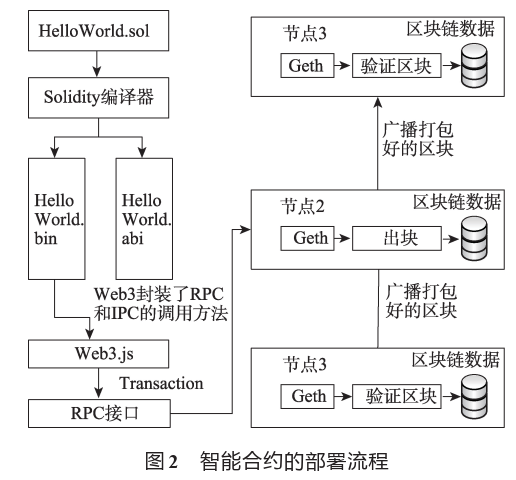
\includegraphics[width=.3\linewidth]{pictures/model_architecture}
    \caption{\label{fig:model_architecture}本研究采用的模型架构}
\end{figure}
\subsection{基于图的注意力掩码}
\label{sec:基于图的注意力掩码}
为了将语义图合并输入到Transformer中,我们遵循原工作\cite{guo2020graphcodebert}引入了基于图的注意力函数来过滤掉不相关的信息。为了在模型中表示语义图中的有向边,以数据流图为例,如果存在有向边$\left\langle v_j,v_i \right\rangle$(即变量$v_i$的值来自变量$v_j$),此时掩码矩阵$M$中对应元素的值为0,\textcolor{red}{那么节点query$q_{v_i}$可以注意到key$k_{v_j}$};否则,掩码矩阵中对应元素的值为$-\infty$,注意力得分${q^T}_jk_i$与之相加并且经过$softmax$函数后计算出的注意力权重变为0,\textcolor{red}{从而避免query$q_j$注意到key$k_i$。}

另一方面,为了表示源代码和数据流之间的关系,我们定义了一个集合$E$记录源代码token$c_j$和变量$v_i$之间的映射关系,即$\left\langle c_j,v_i \right\rangle \in E$表示数据流图中的节点$v_i$和源代码中的token$c_j$相对应。然后,当且仅当$\left\langle c_j,v_i \right\rangle \in E$时,\textcolor{red}{我们允许节点$q_{v_i}$和代码$k_{c_j}$相互参与},用形式化语言描述如下:
\begin{equation}
    M_{ij} =
    \begin{cases}
        0 & \begin{aligned}
               &\text{if } q_i \in \{[CLS], [SEP]\} \text{ or } q_i, k_j \in W \cup C \\
               &\text{or } \langle q_i, k_j \rangle \in E \cup E'
           \end{aligned} \\
        -\infty & \text{otherwise}
    \end{cases}
    \label{eq:mask}
\end{equation}
\textcolor{red}{必要时可扩展一下此章节}

\subsection{训练任务}
\label{sec:训练任务}
除了基本的掩码语言建模(Masked Language Modeling,MLM)任务\cite{devlin2018bert},GraphCodeBert模型中还引入两种全新的预训练任务:数据流边预测和跨源代码与数据流的变量对齐。本文中在数据流图基础上额外引入了控制流图和函数调用图,因此需要在每一类语义图上执行这两种预训练任务,即需要另外添加两类任务:控制流边预测和跨源代码与基本代码块对齐、函数调用边预测和跨源代码与函数名对齐。语义图边的预测任务是为了学习语义图的表示,让模型学习语义图的结构特征;源代码与语义图节点的对齐任务用于将源代码和语义图两种信息联系起来,让模型学习语义图中的节点在源代码中的位置信息。

论文\cite{guo2020graphcodebert}中针对这两类任务提出了对应的损失函数(公式\eqref{loss1}和公式\eqref{loss2}),本文将遵循其设定。
\begin{equation}
loss_{EdgePred}=-\sum_{e_{ij}\in E_{c}}[\delta(e_{ij}\in E_{mask})logp_{e_{ij}}+(1-\delta(e_{ij}\in E_{mask}))log(1-p_{e_{ij}})] \label{loss1}
\end{equation}
\begin{equation}
loss_{NodeAlign}=-\sum_{e_{ij}\in E_{c}^{'}}[\delta(e_{ij}\in E_{mask}^{'})logp_{e_{ij}}+(1-\delta(e_{ij}\in E_{mask}^{'}))log(1-p_{e_{ij}})] \label{loss2}
\end{equation}
% 为了从源代码和数据流图中学习代码表示,他们引入了两种结构感知预训练任务,一种是数据流图的有向边预测任务,用于从数据流图中学习语义信息;另一种是源代码与数据流节点的对齐任务,用于映射源代码中的token与数据流图中的节点,从而保证源代码和数据流图在模型中的语义结构一致。


% 值得一提的是,前文已经阐述了静态代码指标在软件评估工作中的重要性,而且这些指标能在一定维度上表达智能合约的结构信息,因此本文将尝试融合静态代码指标与语义特征,共同训练智能合约的漏洞检测模型,具体内容将在下一小节中阐述。
\subsection{特征融合}
\label{sec:特征融合}
上文描述的基于GraphCodeBERT模型经过预训练后,能针对智能合约源代码和对应的语义图生成高维的上下文表示,而xxx节中计算出的34个静态代码指标在一定维度上表达了智能合约的结构特征,因此如果能将这两种信息融合起来用于智能合约漏洞检测,可能会取得意想不到的效果,接下来将对此进行探究。

常见的融合多种类特征的方法包括直接拼接、联合训练等。Pan等人通过联合语义特征和专家特征训练了一个模型,用于自动识别开发者聊天室中的信息类型,取得了较好的效果。因此,本文也借鉴这种方式,联合静态代码指标和GraphCodeBERT模型生成的表示向量,训练智能合约漏洞检测分类器。

需要注意的是,静态代码指标生成的专家特征是包含34个维度的特征向量,相比于GraphCodeBERT模型生成的语义表示向量具有768个维度。为了避免高维度的语义向量对低维度的专家特征向量形成压倒性优势,本文借鉴了Yang等人的研究成果,利用深度学习技术(本文使用了一个全连接层)对专家特征向量进行嵌入,以获得高纬度的表示向量。如果以$Metrics=\{m_1,m_2,\ldots,m_{34}\}$表示最初计算出的34个专家特征,那么经过全连接层进行嵌入后得到其高维度表示$V_{metrics}=\{\alpha_1,\alpha_2,\ldots,\alpha_t\}$。GraphCodeBERT模型生成的语义表示向量记为$V_{semantic}=\{\beta_1,\beta_2,\ldots,\beta_t\}$,也即公式\eqref{eq5}中的$\hat{G}^n$,在输入分类器时,将$V_{metrics}$和$V_{semantic}$拼接成一个新向量$U=\{\alpha_1,\alpha_2,\ldots,\alpha_t,\beta_1,\beta_2,\ldots,\beta_t\}$,然后在一个全连接层中对其进行fine-tune。

在整个模型的最后,本文使用一个线性分类器,并使用$softmax$函数将结果转换为不同类别的预测概率,如公式\eqref{classifier}所示。
\begin{equation}
\hat{y}=Sigmoid(\hat{U}^{2t}) \label{classifier}
\end{equation}
\section{实验设计与结果分析}
\label{sec:实验设计与结果分析}
描述实验步骤
在预训练阶段,模型学习了如何从图结构中提取有用的信息,并转化为向量表示(Embedding)


\subsection{实验参数及环境}
\label{sec:实验参数及环境}
本文的所有实验的运行环境表\ref{tab:environment}所示。

\begin{table}[htbp]
    \caption{\label{tab:environment}现有工作中使用的数据集的统计信息}
    \small
    \renewcommand{\arraystretch}{1.5}
    \begin{tabularx}{\linewidth}{cX<{\centering}}
        \Xhline{2\arrayrulewidth}
        环境      & 详细信息                                      \\ \hline
        处理器     & Intel(R) Xeon(R) Gold 6226R CPU @ 2.90GHz \\
        内存大小    & 256GB                                     \\
        操作系统    & Ubuntu 20.04.1                            \\
        开发语言    & Python 3.9.6                              \\
        开发工具    & Visual Studio Code                        \\
        深度学习框架  & PyTorch                                   \\
        GPU型号   & NVIDIA GeForce RTX 3090 24GB              \\
        GPU驱动版本 & CUDA 11.4                                 \\ 
        \Xhline{2\arrayrulewidth}
        \end{tabularx}
\end{table}

本文训练了一个包含12层Transformer结构的模型,其中的超参数设定如表\ref{tab:super_parameters}所示。
\begin{table}[htbp]
    \caption{\label{tab:super_parameters}现有工作中的超参设定}
    \small
    \renewcommand{\arraystretch}{1.5}
    \begin{tabularx}{\linewidth}{lX<{\centering}}
        \Xhline{2\arrayrulewidth}
        参数                            & 参数值  \\ \hline
        源代码序列最大长度(code\_length)                  & 256  \\
        数据流序列最大长度(data\_flow\_length)            & 64   \\
        训练批大小(train\_batch\_size)            & 2    \\
        验证批大小(eval\_batch\_size)             & 2    \\
        梯度累积步长(gradient\_accumulation\_steps) & 1    \\
        学习率(learning\_rate)                & 2e-5 \\
        权重衰减系数(weight\_decay)                 & 0.0  \\
        Adam衰减系数(adam\_epsilon)                 & 1e-8 \\
        最大梯度范数(max\_grad\_norm)               & 1.0  \\
        最大训练步数(max\_steps)                    & -1   \\
        学习率预热步数(warmup\_steps)                 & 0    \\
        随机数种子(seed)                          & 42   \\
        训练轮数(epochs)                        & 2    \\ \Xhline{2\arrayrulewidth}
        \end{tabularx}
\end{table}



\subsection{评估指标}
\label{sec:评估指标}
在分类模型中,选用正确的评估标准对模型的度量和评估至关重要,能够及时发现模型的缺陷和可能出现的错误,并根据实际问题不断迭代优化模型。混淆矩阵作为一种可视化工具,通常用于监督学习中比较分类结果和实例的真实标签,反应了分类结果的混淆程度,矩阵的每一列代表实例的真实标签,每一行代表的是预测结果。 如表 4-2 所示,在混淆矩阵中,TP 代表真阳性,表示预测结果和真实结果均为正类;FP 代表假阳性,表示预测结果为正类但真实结果为负类;TN 代表真阴性,表示预测结果和真实结果均为负类;FN 代表假阴性,表示预测结果为负类但真实结果为正类。 
\begin{table}[htbp]
    \caption{\label{tab:confusion_matrix}现有工作中使用的数据集的统计信息}
    \small
    \renewcommand{\arraystretch}{1.5}
    \begin{tabularx}{\linewidth}{cX<{\centering}X<{\centering}X<{\centering}}
        \hline
    数据集名称     & 智能合约数量 & 源代码与字节码 & 时间段            \\ \hline
    smartbugs & 47,518  & 源代码;字节码 & 2015$\sim$2019 \\
    crawID    & 321432 & 源代码     & 2015$\sim$2018 \\
    JiuZhou   & 54325  & 字节码     & 2015$\sim$2018 \\
    xxx       & 5435   & 源代码;字节码 & 2015$\sim$2019  \\  \hline
    \end{tabularx}
\end{table}
对于评估指标,我们采用广泛使用的 Precision、Recall 和 F1-score [7] 、 [17] 。我们选择宏观的方式进行评估,分别计算有漏洞和无漏洞合约的三个指标的值,然后取平均值作为最终结果。这种 a 方式可以反映我们方法的总体性能。
\begin{equation}
\text{F1-score}=2\cdot\frac{\text{Precision}\cdot\text{Recall}}{\text{Precision}+\text{Recal}} \label{f1-score}
\end{equation}
\subsection{实验结果分析}
\label{sec:实验结果分析}
为了验证本文提出的漏洞检测模型的性能,我们将本模型与x种现有的智能合约分析工具进行比较,包括Oyente、Mythril、SmartCheck等等。

\autoref{fig:experiment_result}显示了区块链系统的架构模型。
\begin{figure}[htbp]
    \centering
    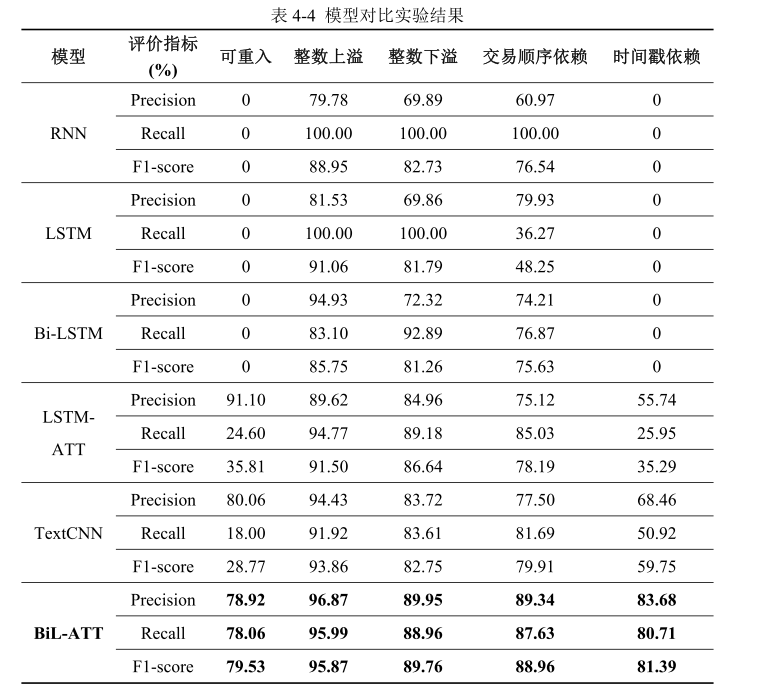
\includegraphics[width=.3\linewidth]{pictures/experiment_result}
    \caption{\label{fig:experiment_result}区块链系统的架构模型}
\end{figure}
从表中可以看出,本文模型的多个多标签评价指标均高于对比模型,体现了 BiLATT 模型在智能合约漏洞多标签检测领域的有效性。RNN 的 micro-R 值较高而 micro-P 较低是因为 RNN 模型发生了严重的过拟合现象,模型更偏向于将样本的漏洞预测为训练集中数量较多的漏洞类别,而其他模型 micro-P 值均高于 RNN 说明我们引入顺序模型 LSTM 对操作码进行处理是明智的,通过对比 LSTM 和 Bi-LSTM 各项指标,证明提取合约操作码之间双向的语义信息更有利于检测合约漏洞,此外,我们还发现 LSTMATT 的各项指标相比 Bi-LSTM 有大幅提升,结合实验过程分析得出注意力机制的加入可以使模型均衡样本数量较少的特征,关注重要的特征数据,对漏洞检测结果的影响相比 Bi-LSTM 起更大作用。TextCNN 是改进的 CNN 模型用于处理 NLP 任务,但是该模型网络结构较为简单,特征提取能力有限,效果表现一般。 

\autoref{fig:experiment_result_chart}显示了区块链系统的架构模型。
\begin{figure}[htbp]
    \centering
    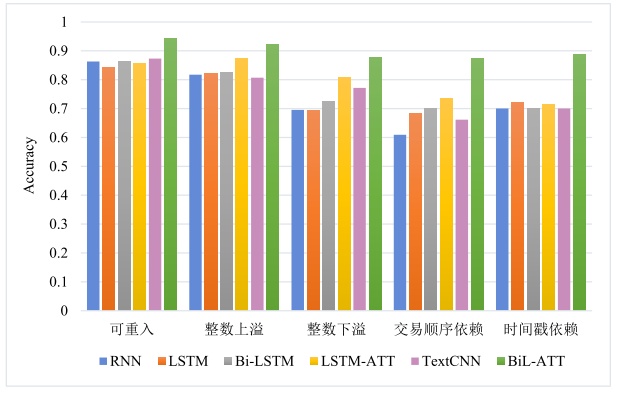
\includegraphics[width=.3\linewidth]{pictures/experiment_result_chart}
    \caption{\label{fig:experiment_result_chart}区块链系统的架构模型}
\end{figure}
图 4-5 所示为六个模型分别对五种漏洞进行检测的 Accuracy 值,Accuracy 值是正确预测的样本数与总样本数的比。可以看出 BiL-ATT 模型对五种漏洞的检测准确率均超过了 85\%,其中可重入漏洞和整数上溢漏洞的准确率超过了 90\%。由于数据集中含有的可重入漏洞和时间戳依赖漏洞的样本数量相较于其他三种漏洞的样本数量较少,因此 RNN 和 LSTM 模型针对这两种漏洞的检测效果看似可观,但实际上,由于这两个模型存在过拟合现象,模型更倾向于预测样本不包含这两个漏洞。通过比较 LSTM 和 BiLSTM 模型,我们可以发现 Bi-LSTM 模型在所有漏洞中的表现都比 LSTM 模型好,说明使用 Bi-LSTM 模型可以有效地提取前后的语义特征,从而更准确地识别漏洞。 

\autoref{fig:experiment_result_table}显示了区块链系统的架构模型。
\begin{figure}[htbp]
    \centering
    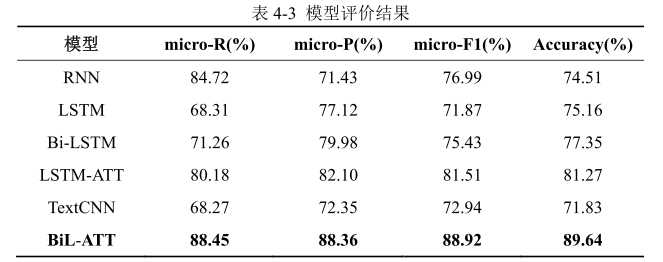
\includegraphics[width=.3\linewidth]{pictures/experiment_result_table}
    \caption{\label{fig:experiment_result_table}区块链系统的架构模型}
\end{figure}
表 4-4 所示为六个模型分别对五种漏洞进行检测的 Precision 值,Recall 值和 F1score,Precision 值可以衡量模型预测出来的样本中被正确预测的数量, Recall 值是用来表示实际样本中有多少被正确预测的数量,F1-score 是统计学中用来衡量二分类模型精确度的一种指标,它同时兼顾了分类模型的准确率和召回率,可以看作是模型准确率和召回率的一种加权平均。从表中可以发现 RNN、LSTM 和 Bi-LSTM 模型都出现了严重的过拟合现象,这是因为训练样本中整数上溢、整数下溢和交易顺序依赖三种漏洞的样本数量远远大于可重入漏洞和时间戳依赖漏洞的数量,模型在不平衡的数据下被训练
地更倾向于样本都包含这三种漏洞,因此这三种漏洞的 Recall 值都为 1,而另外两种样本较少漏洞的 Recall 值为 0。而添加了注意力机制的 LSTM-ATT 模型以及 BiL-ATT 模型,能够合理均衡不同的漏洞,反映出注意力机制可以有效增强模型的泛化能力。由于 TextCNN 模型的网络结构较为简单,因此它也避免了过分拟合漏洞数量较多的漏洞。 BiL-ATT 模型虽然也在样本数量较少的漏洞分类精度不高,在可重入漏洞检测上的 Precision 值仅有 78.92\%,低于 LSTM-ATT 模型和 TextCNN 模型,但是在时间戳依赖漏洞上达到 83.68\%,远高于 LSTM-ATT 模型和 TextCNN 模型,并且在整数上溢、整数下溢和交易顺序依赖这三种漏洞数量较多的样本中,WBL-ATT 模型表现优秀,其 Precision 值大于 TextCNN 模型和 LSTM-ATT 模型。综合来说,BiL-ATT 模型具有较好的泛化性能,能有效地检测智能合约的多种漏洞。 
\subsection{消融实验与结果分析}
\label{sec:消融实验与结果分析}
为了验证本文引入的两种语义图(控制流图和函数调用图)、以及静态代码指标和语义特征融合训练的方法对漏洞检测任务的贡献,本文又在基本实验的基础上增加了消融实验,具体结果如表\autoref{tab:ablation_result}所示。
\begin{table}[htbp]
    \caption{\label{tab:ablation_result}现有工作中使用的数据集的统计信息}
    \small
    \renewcommand{\arraystretch}{1.5}
    \begin{tabularx}{\linewidth}{cX<{\centering}X<{\centering}X<{\centering}}
        \hline
    数据集名称     & 智能合约数量 & 源代码与字节码 & 时间段            \\ \hline
    smartbugs & 47,518  & 源代码;字节码 & 2015$\sim$2019 \\
    crawID    & 321432 & 源代码     & 2015$\sim$2018 \\
    JiuZhou   & 54325  & 字节码     & 2015$\sim$2018 \\
    xxx       & 5435   & 源代码;字节码 & 2015$\sim$2019  \\  \hline
    \end{tabularx}
\end{table}
从表\autoref{tab:ablation_result}中可以看出,当删除控制流图和函数调用图时,模型的整体性能分别从xxx下降到xxx,这表明了更多的语义信息可以提高模型对智能合约的学习能力,提升漏洞检测效果;当删除静态代码指标而只使用语义特征时,模型的整体性能从xxx下降到了xxx,这表明静态代码指标可以在一定程度上反映合约的结构信息,能提升漏洞检测效果。